\chapter{Introduction}
\label{chp:introduction}
Since the introduction of the Internet in the '60s and the world wide web (WWW) in the '90s, more and more people have been connected to each other. Recent research shows that peer-to-peer (P2P) Internet is already back at its prime as it is dominating the traffic as shown in Figure \ref{fig:usage} \cite{2015:internettraffic:sandvine}. User interaction in the Internet community can be expressed in various fashions. Many applications and protocols run on top of P2P system, for instance online gaming, computing, and file sharing. Specifically in file-sharing P2P applications, to ensure all users have a flawless experience, it is necessary to have all peers participate equally. In spite of that, not all of the peers consistently share the file. This phenomenon is called \textit{freeriding}.

\begin{figure}[h]
	\centering
	\begin{subfigure}[b]{0.8\textwidth}
		\includegraphics[width=\linewidth]{pics/sandvineeu2015}
		\caption{Sandvine data for 2015 internet usage in Europe}
		\label{fig:usage1}
	\end{subfigure}\\
	\begin{subfigure}[b]{0.8\textwidth}
		\includegraphics[width=\linewidth]{pics/sandvineasia2015}
		\caption{Sandvine data for 2015 internet usage in Asia Pasific}
		\label{fig:usage2}
	\end{subfigure}%
	\caption{Traffic of the Internet by Sandvine \cite{2015:internettraffic:sandvine}}.
	\label{fig:usage}
\end{figure}

\section{The freeriding phenomenon}
Among all of the peer-to-peer implementations on the Internet, file-sharing is the most popular one. Gnutella was one of the most popular applications from 2000-2007. However, it was shut down because of legal and performance issues. In Gnutella, the majority of users (70\%) stopped sharing their files. Moreover, about half of the requests were served by only the top 1\% of the community \cite{2000:freeridegnutella:adar}. Gnutella suffers from a social phenomenon called \textit{freeriding} with the majority of its users.

Freeriding is defined as user behavior that selfishly consumes all the resources of a system without giving back anything in return. It may cause vulnerabilities in the system \cite{2000:freeridegnutella:adar}. With only a few of the users providing the service for many, it eventually becomes more of a centralized than a decentralized system. It also may degrade system performance \cite{2000:freeridegnutella:adar}. \citeauthor{2000:freeridegnutella:adar} showed that many P2P peers always show self-interest and rationalization that can be considered as freeriding. If freeriders become the majority in a file-sharing peer-to-peer system, they will occupy a significant amount of resources, and eventually bottlenecks in the system will occur. As the time goes on, an honest, important peer may feel dissatisfied and decide to leave the system, taking crucial files with them. The system then becomes degraded, and sooner or later will be completely abandoned by all of its peers.

Freeriding can lead to a systematically worse problem known as ``the tragedy of the commons'' \cite{1968:tragedycommon:hardin}. This problem was popularized by \citet*{1968:tragedycommon:hardin} in \citeyear{1968:tragedycommon:hardin}. This social dilemma emerges because of the overuse and overexploitation of shared resources by the user without any feedback from them. As \citeauthor{1968:tragedycommon:hardin} stated in his paper: ``Freedom in a commons brings ruin to all'', the uncontrolled participants could selfishly take common, limited resource to fulfill their goals.
% how can egoist cooperate :  The Emergence of Cooperation among Egoists (Robert Axelrod). Solved by tit-for-tat -> good performance. managing supply and demand meulpowder p.7

% freerider behaviour, tit-for-tat result
\textit{Extreme freeriding} is a behavior where one does not upload anything while constantly downloading data. Under current standards, this rarely happens. Instead, it is more common to find \textit{hit and run} behavior \cite{2011:managesupplydemand:meulpolder}. Hit and run (HnR) is a situation in which a user finishes downloading, then immediately stops his contribution, i.e uploading \cite{2014:sustainabilitytorrent:chen}. Hit and run is also often cited as one of the freeriding behaviors that peer-to-peer communities want to prevent. 

%Despite of that, hit and run often not directly affects end-user. A recent study stated that freerider in \bt~may not degrade performance as long as the swarm has at least one dedicated and available seeders \cite{2015:freeriderinbtcommunity:das}. 

%. One thing that need to take into consideration is that in their research, they only take four communities as dataset 

\section{BitTorrent protocol}
%\todo{terlalu ribet section ini, better to have a diagram of bittorent dan legend, trus jelasin sedikit aja komponnennya ngapain}
%It survives until now because \bt~ is a \textit{protocol} that can be implemented by anyone, instead of service that Napster, Kazaa, and Gnutella used to have. To build a system on top of \bt~environment, it is essential to know the complete view how \bt~work. 
\bt~\cite{2003:bittorrent:cohen}, nowadays stands as the \textit{de facto} file-sharing protocol on top of the peer-to-peer network. The \bt~protocol can be implemented by anyone, so it is not limited to any particular service such as Gnutella.

% tit-for-tat, choking, unchoke, optimistic unchoke
In the general view, \bt~consists of peers who participate in file-sharing and the \textit{tracker}. The \textit{tracker} is responsible for monitoring the current distribution of files and state of peers in the swarm. The \textit{swarm} is a set of peers formed with the common purpose of downloading or uploading certain files that is represented in the \texttt{.torrent} metadata file. The static \texttt{.torrent} file, which contains information such as tracker addresses and the unique hash value of the swarm it represents, is created by a peer who wants to publish their files. Files in a swarm consist of several \textit{pieces} or file chunks. A piece is exchanged by the peers in a particular period. A \textit{seeder} is a type of peer who has the complete set of files and uploads (or seeds) its pieces to other peers. A \textit{leecher} is a type of peer who downloads from a particular swarm.

%\textit{Tit-for-tat} in \bt~ encourage users to only upload files to one who also has uploaded his file somewhere else. 
%The \textit{tit-for-tat} ranked peer by its upload amount and speed. Therefore, freeriders always get low priority in this mechanism. In this way, \textit{tit-for-tat} incentivizes for user to upload a file.

% how bittorrent handle freeriding (short term)
\bt~uses a \textit{tit-for-tat} mechanism as both reward and punishment method for its peers' behavior. This mechanism is intended to solve the fairness issue introduced by freeriders \cite{2003:bittorrent:cohen}. The \textit{tit-for-tat} mechanism always prioritizes a peer who has uploaded something. \textit{Tit-for-tat} is valid only in a scope of a single swarm. That means the state from one swarm cannot be carried into another swarm. This factor causes \textit{tit-for-tat} to work best only in short term transactions and with limited parties. Nevertheless, \citeauthor{2005:bittorrentcooperation:andrade} showed that \bt~indeed increased cooperation, with less than 6\% of peers having not uploaded anything (extreme freeriding) \cite{2005:bittorrentcooperation:andrade}. As for downloading, \bt~always picks the \textit{rarest piece} first, based on its availability in the swarm. This technique ensures that a complete file is distributed in the swarm.

In order to find the rarest pieces, piece information on peers is necessary. In \bt, there are four methods to discover and update peer information. Those are: using centralized trackers, distributed hash table (DHT), peer exchange (PEX), and local service discovery (LSD). Towards a ``trackerless'' \bt~system, DHT allows each peer to become a tracker. LSD is specialized to find peers in a local network. PEX is a mechanism to efficiently contact a peer directly to exchange up-to-date information.

There are many \bt~\textit{communities} that serve as portals to store \texttt{.torrent} files. In general, a community in \bt~ can be divided into two categories: \textit{public} and \textit{private}. A public community is one in which everybody can join the swarm served by a tracker in that community. On the other hand, private communities are closed communities which can only be accessed by passing a particular requirement \cite{2010:pubpriv:meulpolder, 2014:sustainabilitytorrent:chen}. Typically, private communities have higher performance compared to public communities \cite{2010:pubpriv:meulpolder}. \citeauthor{2010:pubpriv:meulpolder} measured that private communities have 3 to 5 times faster download speeds than public communities \cite{2010:pubpriv:meulpolder}. \textit{Private communities} typically have higher seeder-to-leecher ratio (SLR) that affects the download speed \cite{2005:bittorrentcooperation:andrade}. In such a community, the administrator may enforce a policy such as \textit{Share Ratio Enforcement} (SRE). SRE defines the amount a user needs to upload before being able to download from the community \cite{2012:economicbt:kash}. 
Higher performance comes with a drawback: in private communities, it is very difficult to obtain a new membership and also very easy to be kicked out \cite{2013:survivepriv:jia}.

\subsection{Tribler}
\label{section:tribler}
%\todo{taruh diagram lagi supaya enak dibaca, komponen kaya end-to-end encrption, dispersy, jadiin kotak aja trus tulis di legend}
Tribler\footnote{\url{https://www.tribler.org/}} is peer-to-peer file sharing application developed at the Delft University of Technology that is compatible with the \bt~protocol \cite{2008:tribler:pouwelse}. Tribler is a fully decentralized system focused on security and anonymity. Starting with ABC (Another \bt~Client), Tribler currently provides content discovery, channels concept, and reputation management in a fully distributed manner. Tribler was downloaded from the official repository on the latest stable release (6.5.2) as many as 172716 times\footnote{\url{http://www.somsubhra.com/github-release-stats/ ?username=tribler&repository=tribler} (Accessed 7 February 2017)}.

All of Tribler's main components (such as end-to-end encryption, channel discovery, and many others) rely upon a database and dissemination system called \texttt{Dispersy} \cite{2013:dispersy:zeilemaker}. Dispersy maintains and performs the communication functions between Tribler peers in a fully decentralized manner. Dispersy can circulate the message in one-to-one or one-to-many within a group of nodes called a \textit{community}. Important \textit{communities} are summarized in Table \ref{tbl:community} \cite{2016:tribler-techdebt:vos}. We would like to focus on the \textit{channel} community, which is a community to distribute swarms among Tribler users. Each user can create their own \textit{channel}, add and remove torrents to it, and maintain its activity. 

%Users can adapt and implement its desired \textit{community} by itself. It is including how, what, and where the communication will occur.

\begin{table}[tbp]
	\centering
	\caption{Overview of implemented Dispersy community in Tribler \cite{2016:tribler-techdebt:vos}.}
	\label{tbl:community}
	\begin{tabular}{|c|p{11cm}|}
		\hline
		\rowcolor[HTML]{EFEFEF} 
		\multicolumn{1}{|c|}{\cellcolor[HTML]{EFEFEF}{\color[HTML]{333333} \textbf{Community Name}}} & \multicolumn{1}{c|}{\cellcolor[HTML]{EFEFEF}{\color[HTML]{333333} \textbf{Purpose}}}                                                                                                                                     \\ \hline
		\textit{AllChannel}                                                                          & Used to discover new channels and to perform remote channel search operations.                                                                                                                                           \\ \hline
		\textit{BarterCast4}\cite{2009:bartercast:meulpolder}                                                                         & While currently disabled, this community was used to spread statistics about the upload and download rates of peers inside the network and was originally created as a mechanism to prevent freeriding in Tribler. \\ \hline
		\textit{Channel}                                                                             & This community represents a single channel and is responsible for managing torrents and playlists inside that channel.                                                                                                   \\ \hline
		\textit{Multichain}          \cite{2015:multichain:norberhuis}                                                                & This community utilizes the blockchain technology, and can be regarded as the accounting mechanism that keeps track of shared and used bandwidth.                                                                         \\ \hline
		\textit{Search}                                                                              & This community contains functionalities to perform remote keyword searches for torrents and torrent-collecting operations.                                                                                               \\ \hline
		\textit{(Hidden)Tunnel}                                                                      & This community contains the implementation of the Tor-like protocol that enables anonymity when downloading content and contains the foundations of the hidden seeder services protocol, used for anonymous seeding.     \\ \hline
	\end{tabular}
\end{table}

%Tribler implements several Dispersy \textit{communities} on its core function. \citeauthor{2016:tribler-techdebt:vos} summarize the communities in Tribler. Important features such as channel discovery, search within communities, end-to-end Tor-like operations, and currency mechanism are shown in table \ref{tbl:community}. \textit{Channel} is a collection of torrent that has extra capabilities such as vote system, spam prevention, and comment (social) attributes. 

\section{Rewarding user contribution}
\label{sec:userreward}

\bt~is not enough to tackle HnR behavior. Usually, it is necessary to introduce another layer of rewarding scheme, called the \textit{incentive mechanism}. Incentive mechanism is a method to reward the user for their contribution. In some cases, it also fines users for misconduct. SRE in private communities is a good example of an incentive mechanism, which increases user contribution and swarm performance. It proves that freeriding behavior can be prevented by the use of a proper incentive mechanism. For showing goodness, specifically by uploading data to others, users should get a reward. However, users are typically selfish and always try to maximize their benefit \cite{2015:incentivep2pgame:kang}.

An incentive mechanism is essential as it is one of the properties by which general performance is increased. \citeauthor{2011:managesupplydemand:meulpolder} discussed several kinds of incentive mechanisms that can be combined and complement each other. These are : (i) direct reciprocity, (ii) indirect reciprocity, (iii) centralized reputation, (iv) decentralized reputation, and (v) currency \cite{2011:managesupplydemand:meulpolder}. \textit{Reciprocity} is focused on the relationship between peers. As shown in \ref{fig:reciprocation}, it is classified into two categories: \textit{downstream} and \textit{upstream}. \textit{Reputation} mechanism is more straightforward. The information of user behavior in the past is stored (either centralized or decentralized). This information is iteratively updated and spread through all the peers. The last mechanism is \textit{currency} which uses \textit{credit} to incentivize the user. In theory, it can emulate other incentive mechanisms by quantifying reputation/help. Because of its wide applicability, we will focus on improving the \textit{currency} mechanism.  A \textit{private community} with SRE is the most common implementation of the currency mechanism. 

\begin{figure}[t]
	\centering
	\includegraphics[width=0.7\textwidth]{pics/reciprocation.pdf}
	\caption{Direct and indirect reciprocation}
	\label{fig:reciprocation}
\end{figure}

The \textit{currency} mechanism uses the concept of \textit{credit} as a transaction unit. Therefore, it is often referred as the \textit{credit system}. Users need to \textit{buy} the content and can get \textit{credit} by providing service such as uploading data to others. ``Wealth'' is a collection of stored credit with a particular user. The ``price'' of a file is the amount of credit deducted from a downloader's wealth. Credit might be asymmetrical as shown by \citeauthor{2012:economicbt:kash}\cite{2012:economicbt:kash}. Credit can also depend on the importance. For example, seeding more swarms, seeding longer and old swarms, and seeding swarms that consume large disk space \cite{2014:sustainabilitytorrent:chen}. \citeauthor{2012:economicbt:kash} suggest that a community should carefully declare different prices for different files. One way to do this is by lowering the price for old content, or by defining price depending on its availability and swarms' capacity \cite{2012:economicbt:kash}. However, in this work, we will assume that the credit is unrelated to the file content. It only depends on the bytes transferred between peers.

% incentive in p2p example
There have been several attempts to invent an incentive mechanism. \citeauthor{2015:incentivep2pgame:kang} proposed an incentive mechanism for dynamic and heterogeneous peers using game theory. In their system, each peer can set a price for the service it provides. The buyer (downloader) is then able to negotiate with the seller (uploader) regarding the content price and its bandwidth allocation \cite{2015:incentivep2pgame:kang}. In another research, \citeauthor{2010:effortincentive:rahman} proposed effort-based incentive to advocate fairness between peers \cite{2010:effortincentive:rahman}. In this system, the user is rewarded based on their effort, which is relative to their capacity. Currently, none of these researches are widely applicable. It either needs modification on the protocol or only works under a certain type of application. Nowadays, the users who want to get credit may need to be on standby for a long time waiting for someone to download their files \cite{2013:survivepriv:jia}. Ironically, this approach is inefficient and wastes bandwidth, but is commonly in practice\cite{2013:survivepriv:jia}.

\section{Thesis structure}
Our objective is to establish a layer, namely the credit mining system, on top of the existing currency system in order to lessen the hit and run (HnR) effect on \bt~communities, and to automatically let users gain credit efficiently by uploading only necessary data. Both of these purposes are directed at one vision : improving performance on \bt~communities. The system is intended to work without the need to change the existing, widely implemented credit system.

This thesis is structured as follows. Chapter 2 discusses the specific problem that we intend to solve. Chapter 3 presents the design of the credit mining system and its requirements. Chapter 4 shows the core investment algorithm we proposed. Implementation of the mechanism and its experiment setup will be elaborated in chapter 5. Chapter 6 shows the performance of the credit mining system. Chapter 7 then concludes the work and mentions possible future work.


